

%========
% FIGURES 
%========

\newcommand{\BraggFigureNum}{
\begin{figure}
\centering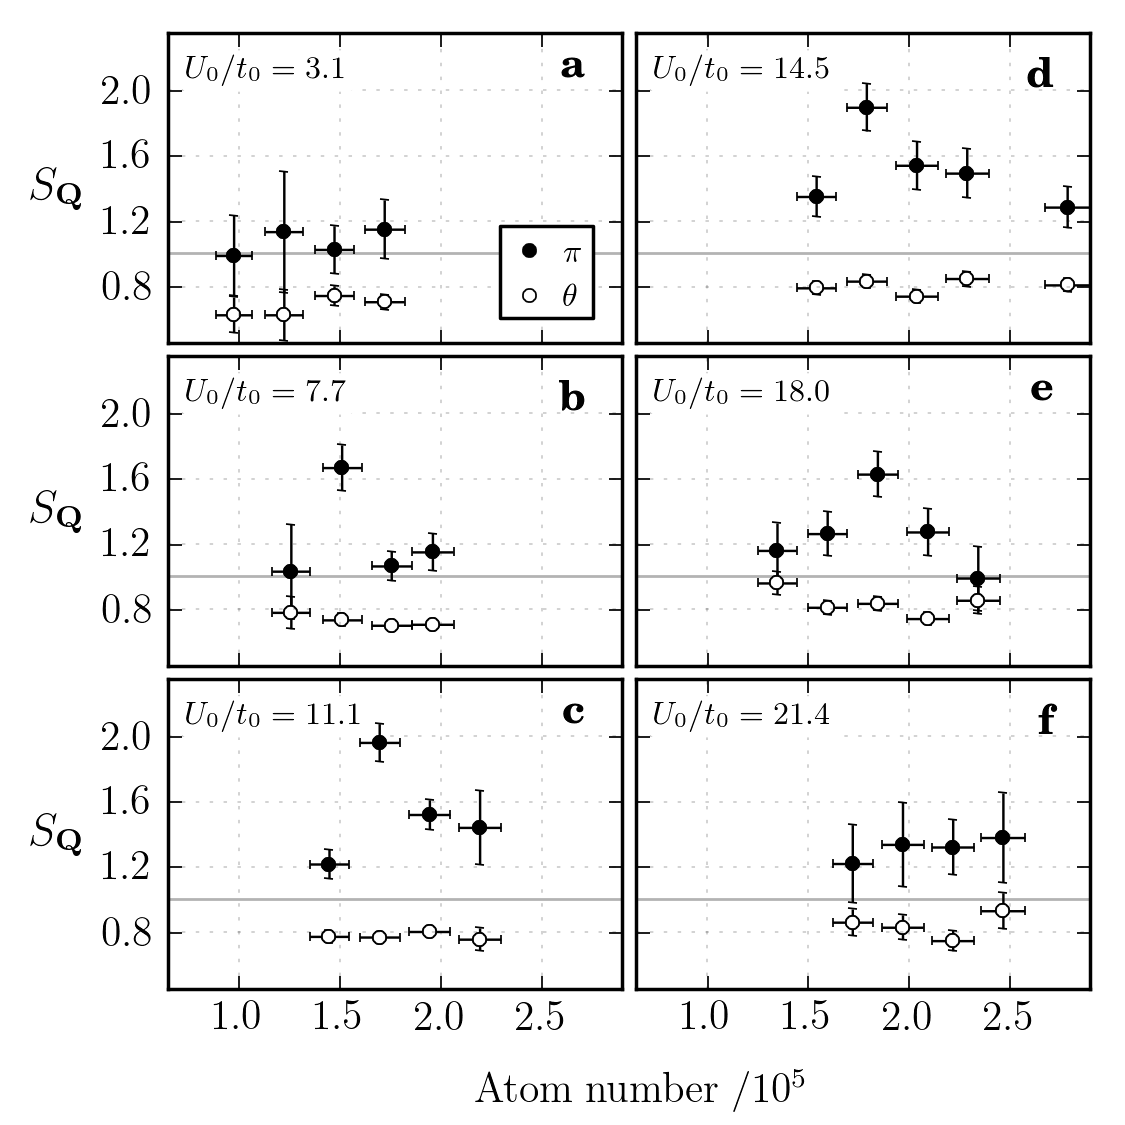
\includegraphics[width=0.8\textwidth]{../figures/afmpaper/03_SvsN.png}
\caption{ \textbf{Spin structure factor as a function of $N$.} \textbf{a-f},
For each $U_{0}/t_{0}$ we vary the atom number $N$ loaded into the lattice and
measure $S_{\bv{\pi}}$ and $S_{\bv{\theta}}$, (closed and open circles,
respectively).   We find that $S_{\bv{\pi}}$ depends sensitively on $N$ for all
but the lowest and highest values of $U_{0}/t_{0}$, where $S_{\bv{\pi}}$ is
near 1. This sensitivity is consistent with the assumption that only a small
volume with $n\simeq1$ mainly contributes to $S_{\bv{\pi}}$. The peak in
$S_{\bv{\pi}}$ shifts to higher $N$ with increasing $U_{0}/t_{0}$ since the
global chemical potential to realize $n=1$ at the center grows with
$U_{0}/t_{0}$.  Vertical error bars represent the standard error of the mean of
at least 15 and up to 60 measurements; more measurements were taken at the peak
of $S_{\bv{\pi}}$.  Horizontal error bars represent the standard error of the
mean of at least 20 measurements of $N$.    }
\label{fig:bfig03}
\end{figure}
}


%%%%%%%%%%%%%%%%%%%%%%%%%%%%%%%%%%%%%%%%%%%%%%%%%%%%%%%%%%%%%%%%%%%%%%%%%%%%%%%
%%%%%%%%%%%%%%%%%%%%%%%%%%%%%%%%%%%%%%%%%%%%%%%%%%%%%%%%%%%%%%%%%%%%%%%%%%%%%%%
%%%%  CHAPTER AFM 
%%%%%%%%%%%%%%%%%%%%%%%%%%%%%%%%%%%%%%%%%%%%%%%%%%%%%%%%%%%%%%%%%%%%%%%%%%%%%%%
%%%%%%%%%%%%%%%%%%%%%%%%%%%%%%%%%%%%%%%%%%%%%%%%%%%%%%%%%%%%%%%%%%%%%%%%%%%%%%%
\chapter{Antiferromagnetic correlations in the Hubbard model}
\label{chap:afmbragg}

The contents of this chapter are based on  a paper that has been submitted for
publication, titled ``Observation of antiferromagnetic correlations in the
Hubbard model with ultracold atoms''~\cite{Hart2014arxiv}. 

For this experiment we realize the Hubbard model in a 7\,$E_{r}$ lattice with
repulsive interactions.  We vary the interaction strength $U_{0}/t_{0}$ in the
range $3.1 < U_{0}/t_{0} < 21.4$.  For each value of the interaction strength
we measure the spin structure factor of the system, \sq,  as a function of atom
number, in the range of 1$\times 10^{5}$ to 2.5$\times 10^{5}$ atoms.  We find
that, for a momentum transfer $\bv{Q}=\bv{\pi} \equiv \frac{2\pi}{a}\hhh$,
which  satisfies the Bragg condition for scattering from a magnetically ordered
sample,  \sPi\ shows a maximum with respect to atom number.   We plot the
maximal \sPi\ vs.  $U_{0}/t_{0}$,  and compare the data to the results of
numerical calculations at different temperatures.   From the comparison we can
quantitatively extract the temperature of the system in a regime previously
unexplored with ultracold atoms, where the entropy is mostly contained in the
spin degree of freedom.

\section{Experimental setup}

\begin{figure}
\begin{center}
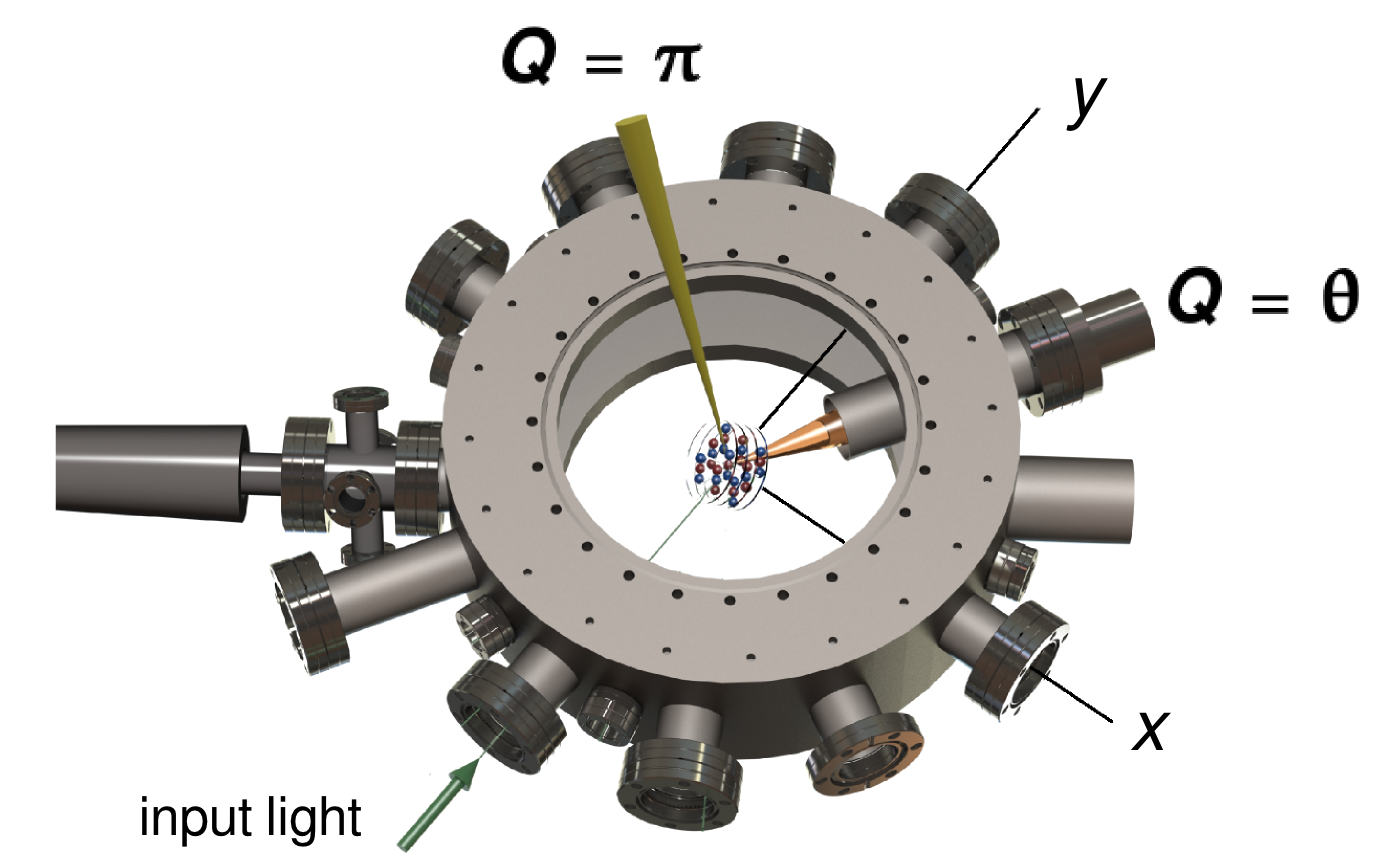
\includegraphics[width=90mm]{../figures/afmpaper/chamber-setup.png} 
\end{center}
\caption{\textbf{Experimental setup used for Bragg scattering.} Light is
collected on directions corresponding to momentum transfers
$\mathbfsf{Q}=\bv{\pi}$ and $\mathbfsf{Q}=\bv{\theta}$.  The $x$ and $y$ axes
of the coordinate system (right handed) are shown.  A bias magnetic field,
which sets the quantization axis and the interaction strength, points in the
$z$ direction.   The input Bragg beam lies in the $yz$ plane, and its
wavevector makes an angle of 3$^{\circ}$ with the positive $y$ axis.  }
\label{fig:bfig1}
\end{figure}


As was mentioned in Chapter~\ref{chap:bragg-scatt}, we obtain spin sensitivity
by setting the Bragg laser frequency between the optical transition frequencies
for states $|1\rangle$ and $2\rangle$.  We measure the spin structure factor
for two values of the momentum transfer $\bv{Q}$, which are labeled $\bv{\pi}$
and $\bv{\theta}$, and are illustrated in Fig.~\ref{fig:bfig1}.   The Bragg
condition is satisfied for $\bv{Q}=\bv{\pi}$ but not for $\bv{Q}=\bv{\theta}$,
so the results at $\bv{\theta}$ serve as a control for the experiment.    The
components of the momentum transfers $\bv{\pi}$ and $\bv{\theta}$ are 
\begin{align*} \bv{\pi} & =\frac{2\pi}{a}(-0.5,-0.5,+0.5) \\
\bv{\theta} & =\frac{2\pi}{a}(+0.396,-0.105,-0.041).
\end{align*} 
 
The spin structure factor, \sq, is obtained by first locking the lattice to a
depth of 20\,$E_{r}$ and then measuring the ratio of the scattered intensity
\textit{in-situ} (denoted $I_{\bv{Q}0}$) to the scattered intensity after a
time-of-flight $\tau=6\,\mu$s following release from the lattice (denoted
$I_{\bv{Q}\infty}$).  As was mentioned in Chapter~\ref{chap:bragg-scatt}, it is
important to include the effects of saturation of the atomic transition when
obtaining the spin structure factor from the measured intensities. Here, the
Bragg probe beam is a collimated Gaussian beam, with a $1/e^{2}$ radius of
$450\,\mu$m and power of $250\,\mu$W.  The saturation parameter is $s_{0}=15.5$
and the detuning (in units of $\Gamma$) is $|\Delta|=6.4$, which results in a
correction due to saturation effects 
\begin{equation}
  1 + \frac{s_{0}}{4\Delta^{2}} = 1.09.
\end{equation} In addition, one must include the Debye-Waller correction due to
the finite extent of the atomic wavefunctions in the 20\,$E_{r}$ lattice.   We
have respectively (cf. Eq.~\ref{eq:define-debyew}) 
\begin{align*}
 e^{2W_{\bv{\pi}}(\tau=0) }& = \exp\left[ \frac{3}{2\sqrt{v_{0}/E_{r}}} \right]
= 1.40 \\ e^{2W_{\bv{\theta}}(\tau=0)} & = 1.08 
\end{align*}
 
\sq\ is obtained from the scattered intensities by using 
\begin{equation} 
\boxed{
 \sq =  1 + C_{\bv{Q}}  
   \left( \frac{ I_{\bv{Q}0} }{ I_{\bv{Q}\infty}} - 1 \right) }
\vspace{0.8em}
\label{eq:correction-sq}
\end{equation}
where $C_{\bv{Q}}=e^{2W_{\bv{Q}}(\tau=0) }\left( 1 + \frac{ s_{0} }{ 4
\Delta^{2} } \right)$ is the correction factor, with values
\begin{align*}
 C_{\bv{\pi}} & = 1.52 \\ 
 C_{\bv{\theta}} & = 1.18  
\end{align*}
for $\bv{\pi}$ and $\bv{\theta}$ respectively. 

\subsection{Light collection.} We collect Bragg scattered light in the
$\bv{\pi}$ direction over a full angular width of  110~mrad,  given by a 2.5
cm diameter collection lens located 23 cm away from the atoms.    In the
$\bv{\theta}$ direction, light is collected by a 2.5 cm diameter  lens
placed 8 cm away from the atoms, corresponding to a full angular width of
318~mrad.  The scattered light in each of the directions is focused to a few
pixels on the cameras, so no additional angular information is obtained.
For $N=1.8\times10^{5}$, $s_{0}=15.5$, $\Delta=6.4\,\Gamma$ and a
$1.7\,\mu\text{s}$ pulse, the detector in the $\bv{\pi}$ direction collects
approximately 1300 photons, whereas the detector in the $\bv{\theta}$
direction collects approximately $10^4$ photons.   The noise floor from
readout, dark current and background light per shot has a standard deviation
equivalent to approximately 250 photons in the $\bv{\pi}$ direction and 1000
photons in the $\bv{\theta}$ direction\footnote{Note that we perform
background subtraction using the eigenface method~\cite{PhysRevA.82.061606}.
The noise floor is determined from the standard deviation of a set of shots
without any atoms.}.

\subsection{Data averaging.} The signals we detect are small enough that an
uncorrelated sample may, in a single shot, produce a scattering signal as
large as the ones produced by samples with AFM correlations.  To obtain a
reliable measurement of $S_{\bv{\pi}}$ we average at least 40
\textit{in-situ} shots to obtain $I_{\bv{Q}0}$ and at least 40
time-of-flight shots to obtain $I_{\bv{Q}\infty}$.
 
We estimate the expected variance on $S_{\bv{\pi}}$ by considering a
randomly ordered sample in which
$e^{i\bv{\pi}\cdot\bv{R}_{n}}2\langle\sigma_{z}\rangle_{n} $  is equal to +1
or -1 with equal probability.  $S_{\bv{\pi}}$ can be written as
\begin{equation*}
  S_{\bv{\pi}} =
    \left| \sum_{n} e^{i\bv{\pi}\cdot \bv{R}_{n}}
    \frac{2 \langle \sigma_{z}  \rangle_{n} }{\sqrt{N}}  \right|^{2}, 
\end{equation*}
which is equivalent to the square of the distance traveled on an unbiased
random walk with step size $1/\sqrt{N}$.   The mean and standard deviation can
then be readily calculated: $\overline{S_{\bv{\pi}}}=1$ and
$\sqrt{\text{Var}(S_{\bv{\pi}})}=\sqrt{2}$, where $\text{Var}(S_{\bv{\pi}})$
denotes the variance of the random variable $S_{\bv{\pi}}$.  With a standard
deviation that is larger than the mean value, a considerable number of shots
needs to be taken in order to obtain an acceptable error in the mean.    The
standard error of the mean for 40 shots will be $\sqrt{2/40}=0.22$, nearly
consistent with what we obtain in the experiment (cf. vertical error bars in
Fig.~\ref{fig:bfig4}).

\subsubsection{Expected variation when $\overline{S_{\bv{\pi}}} > 1$}

We can generalize the above ideas for the situation when
$\overline{S_{\bv{\pi}}} > 1$.  In that case the spin structure factor can
be thought of as the square of the magnitude of a \textit{biased} random
walk (as opposed to \textit{unbiased} as above).  Consider the random
variable $X_{N}$, which represents the total distance traveled in a random
walk with unit step after $N$ steps.  The probability of taking a positive
step is $p$ and the probability of taking a negative step is $1-p$. The spin
structure factor for momentum transfer $\bv{\pi}$ can be written as  
\begin{equation*}
  S_{\bv{\pi}}(p) = \frac{1}{N}  X_{N}^{2}  
\end{equation*}
The unbiased random walk, which gives $\overline{S_{\bv{\pi}}}=1$,
corresponds to $p=0.5$.  A perfectly ordered sample corresponds to $p=1$ or
$p=0$, in which case $X_{N}^{2}=N$ and $S_{\bv{\pi}}=N$.

We can obtain the mean and the variance of $S_{\bv{\pi}}(p)$, as a function
of $p$, from the known properties of a biased random walk.  The probability
distribution for $X_{N}$ is a binomial distribution: 
\begin{equation}
  P(X_{N}=k) = \binom{N}{ (N+k)/2 } p^{(N+k)/2} (1-p)^{(N-k)/2} 
\end{equation}
which in the limit of a large number of steps can be approximated by a
Gaussian probability distribution.  Defining $q=1-p$ this is
% I got this result from http://www.math.uah.edu/stat/bernoulli/Walk.html
\begin{equation}
  P(X_{N}=k) =  \frac{1}{\sqrt{2\pi}\sqrt{4 N pq}} 
\exp\left[ -\frac{1}{2}\frac{(k-N(p-q))^{2}}{4 N pq }  \right]
\end{equation}
The probability distribution for $X_{N}^{2}$ can be obtained from $P(X_{N}=k)$ as 
\begin{equation}
\begin{split}
  P( X_{N}^{2} = k^{2} ) & = \frac{1}{2\sqrt{k^{2}}} [P( X_{N}=k)+P(X_{N}=-k)] \\
   & =
 \frac{1}{2\sqrt{k^{2}}} 
   \frac{1}{\sqrt{2\pi}\sqrt{4 N pq}} 
  \left(
\exp\left[ -\frac{1}{2}\frac{(\sqrt{k^{2}}-N(p-q))^{2}}{4 N pq }  \right]\right. \\
 & ~~~~~~~~~~~~~~~~~~~~~~~~~~~~~~~~~~ + \left.
\exp\left[ -\frac{1}{2}\frac{(-\sqrt{k^{2}}-N(p-q))^{2}}{4 N pq }  \right]  \right)
\end{split}
\end{equation}

We can go one step further and calculate the probability distribution for
$S_{\bv{\pi}}$, for which we obtain
\begin{equation}
\begin{split}
  P( S_{\bv{\pi}} = s ) & = \frac{\sqrt{N}}{2\sqrt{s}} 
     \left[ P( X_{N}=\sqrt{sN}) + P( X_{N}=-\sqrt{sN}) \right] \\
   & =
   \frac{\sqrt{N/s}}{2\sqrt{2\pi}\sqrt{4 N pq}}
   \left( 
    \exp\left[ -\frac{1}{2}\frac{(\sqrt{sN}-N(p-q))^{2}}{4 N pq }  \right] \right. \\ 
& ~~~~~~~~~~~~~~~~~~~~~~~~~~~~~~~~~~~ \left.
 +   \exp\left[ -\frac{1}{2}\frac{(-\sqrt{sN}-N(p-q))^{2}}{4 N pq }  \right]
   \right)
\end{split}
\label{eq:probSpi}
\end{equation}

The mean and variance of this probability distribution can be calculated
analytically by doing the integrals in Mathematica,  the results are
\begin{equation}
\begin{split} 
  \text{Mean}( S_{\bv{\pi}} ) & = N(2p-1)^{2} + 4pq \\ 
  \text{Var}( S_{\bv{\pi}} ) &  = 16pq( N(2p-1)^{2} + 2pq ) 
\end{split}
\end{equation}

For $p=0.5$ we obtain the results of the previous section, namely
$\sqrt{\text{Var}(S_{\bv{\pi}})}=\sqrt{2}$.  For an experimentally measured
$\overline{S_{\bv{\pi}}}\equiv \bar{s} > 1$, we simply need to find $p$ such
that $\overline{S_{\bv{\pi}}} = \bar{s}$,  and then we can calculate
the expected variance.   

For example,  for $\bar{s}=2$ (close to the largest spin structure factor that
we measure in the experiment, cf. Fig.~\ref{fig:bfig4}) and
$N=1.7\times10^{5}$~atoms  we have $p=0.4988$ or $p=0.5012$.   For either $p$,
the resulting standard deviation is
$\sqrt{\text{Var}(S_{\bv{\pi}})}\approx\sqrt{6}$.  The ratio of the standard
deviation to the mean is $\sqrt{6}/2=1.22$, lower than in the completely random
(unbiased) case, where it is $\sqrt{2}$.  We observe that the standard error of
the mean for a set of 40 shots would be given by  $\sqrt{6/40} = 0.38$,  about
one and a half times larger than what we found in the unbiased case.

In Fig.~\ref{fig:spi-noise} we present results for the mean and the standard
deviation for a few values of $p$ and $N =1.7\times10^{5}$~atoms.

\begin{figure}
\centering
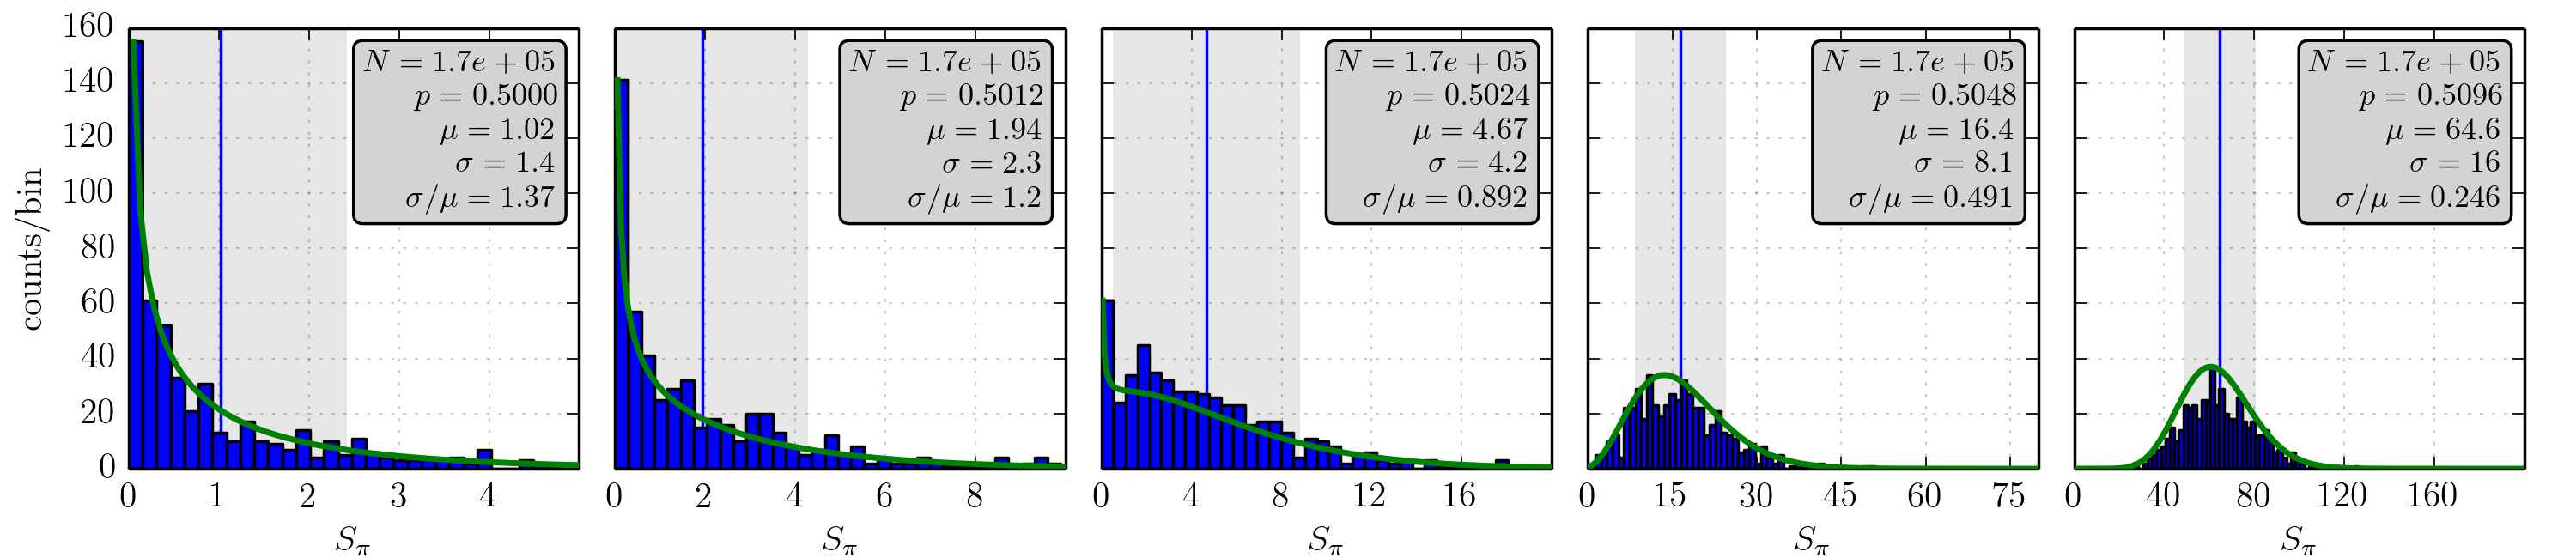
\includegraphics[width=\textwidth]{../figures/braggscatt/Noise_hist.png}
\caption[Fluctuations in $S_{\bv{\pi}}$]{\small Distribution of $S_{\bv{\pi}}$
for randomly ordered spins with bias probability given by $p$ (as described in
the text $p=0.5$ corresponds to a completely random sample, and $p=0$ or $p=1$
correspond to a completely ordered sample.).   The histograms resulting of 520
numerical realizations of the random walk are shown in blue.  The vertical line
denotes the mean of the numerically generated distribution ($\mu$ in the figure
legends) and the shaded gray area denotes $\pm1$ standard deviations ($\sigma$
in the figure legends). The probability distribution $P(S_{\bv{\pi}})$ as
derived in the text (Eq.~\ref{eq:probSpi}) is shown by the green line.  As the
sample becomes ordered, the ratio $\sigma/\mu$ decreases.  The situation that
most closely resembles our experimental results is shown in the second panel,
where $p=0.5012$, which results in $\overline{S_{\bv{\pi}}}\approx 1.94$ (cf.
Fig.~\ref{fig:bfig4}).}
\label{fig:spi-noise}
\end{figure}

\subsection{Other considerations for Bragg scattering} 

\paragraph{Momentum transferred from the probe to the atoms.}

In the derivation of the relationship between the intensity and the structure
factor, showed in Chapter~\ref{chap:bragg-scatt}, we assumed that the center of
mass state of the atom remains unchanged after scattering a photon.  For this
assumption to be valid, the Lamb-Dicke  parameter, $\eta^{2}$, which is defined
as the ratio between the recoil energy of the scattered photon to the harmonic
oscillator spacing in a lattice site\footnote{  \begin{equation} \eta^{2}=
E_{r,\text{probe}} /( 2E_{r} \sqrt{v_{0}/E_{r}})\end{equation} where
$E_{r,\text{probe}}$ is the recoil energy for light at the probe wavelength,
and $v_{0}$ is the lattice depth. Since
$\lambda_{\mathrm{p}}=671\,\mathrm{nm}$, we have $E_{r,\text{probe}} /E_{r} =
1064^{2}/671^{2}=2.514$ } , needs to be $\eta^{2} \ll 1$.  In the locked
20\,$E_{r}$ lattice, $\eta^{2}= 0.27$, meaning that approximately one out of
every 4 photons scattered will excite an atom to the second band of the
lattice.    An atom in the second band has larger position variance and
therefore a smaller Debye-Waller factor,  so it contributes less to the Bragg
scattering signal.

The total number of photons scattered is given by  $t_{\text{exp}} \Gamma
\frac{s_{0}/2}{s_{0} + 4\Delta^{2}+1 }$,  where the duration of the probe pulse
is $t_{\text{exp}}=1.7\,\mu$s and the linewidth of the excited state is
$\Gamma=1/27.1$\,\,ns$^{-1}$~\cite{McAlexander1996}.  For $s_{0}=15.5$ and
$\Delta = 6.4$ this corresponds to 2.7 photons scattered per atom during the
probe pulse.   In a 20\,$E_{r}$ lattice it is then somewhat justifiable to
assume the atoms remain in the lowest band during the pulse.  Since recoiling
to the second band is a single atom process, this effect occurs for all values
of the momentum transfer.  In this work we have not corrected for any effects
due to heating of the atoms to the second band during the duration of the probe
pulse.  It is clear that in the absence of such a correction our measurement
underestimates the value of the spin structure factor in the system.  

For the Bragg scattering measurements performed after time-of-flight, the
momentum transferred from the probe to the atoms plays a more significant role,
since the atoms are not trapped and will recoil after every photon scatter.  As
we will show below (cf. Fig~\ref{fig:bfig2}), we still see good agreement
between the observed decay of the Bragg scattering signal in time-of-flight and
the decay expected for a Heisenberg limited wavepacket
(Eq.~\ref{eq:bragg-tof-decay}).   A similar consideration arises for Bragg
scattering off of the \zoz\ lattice planes,  where in
Chapter~\ref{chap:bragg-scatt} we saw that there was also good agreement with
Eq.~\ref{eq:bragg-tof-decay}.  


\paragraph{Optical density.} A low optical density of the sample is important
so that the probe is unattenuated through the atom cloud, and multiple
scattering events of the Bragg scattered photons are
limited~\cite{Ted2010}.  The optical density  can be approximated as
\begin{equation*}
   \text{OD}
  \simeq
    \frac{ \sigma_{0} | \bv{\hat{e}}_{\text{p}} \cdot \bv{\hat{e}}_{-1} |^{2}}
         {  4 \Delta^{2} + s_{0} }
    \frac{1}{a^{2}}
    \left(\frac{ 3N}{4\pi} \right)^{1/3}
\end{equation*}
where $\sigma_{0}=3\lambda_{0}^{2}/2\pi$.  With $s_{0}=15.5$,
$\Delta=6.4$  and $N=1.8\times10^{5}$ atoms we have
$\text{OD}\simeq0.072$\,.  At this value we do not expect significant
corrections to the spin structure factor measurement due to the attenuation of
the probe.  We do not include any corrections in our measurement due to
finite optical density effects. 


\section{Time-of-flight}
 
\begin{figure}
\centering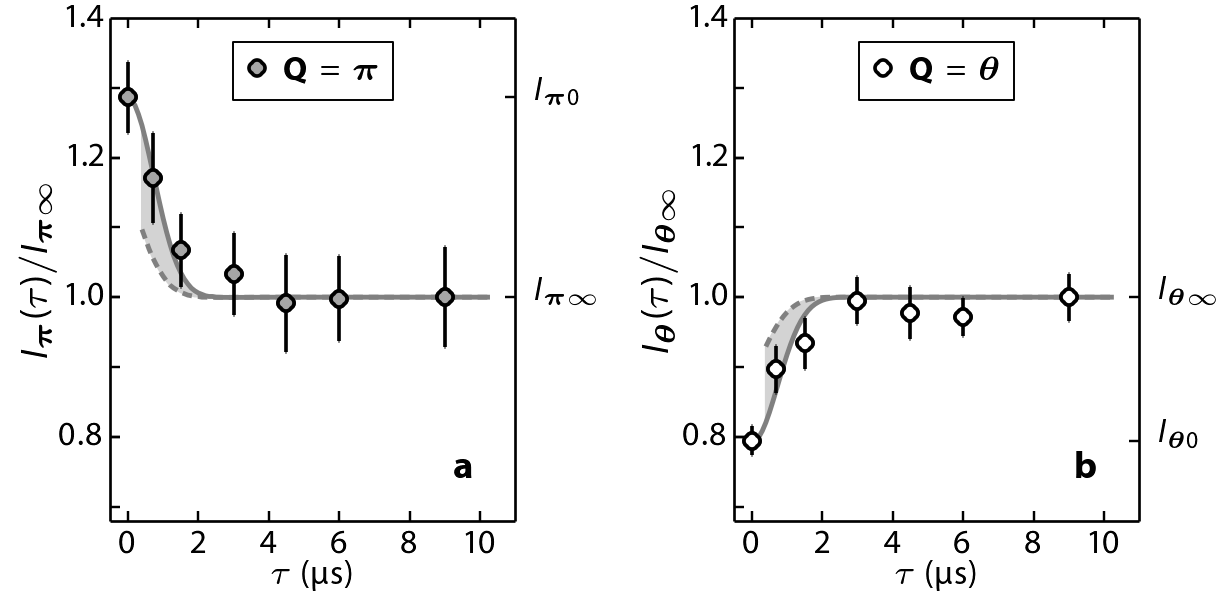
\includegraphics[width=0.8\columnwidth]{../figures/afmpaper/Hulet_fig2.png}
%
\caption{\textbf{Time-of-flight measurement of scattered intensity from a
sample with AFM correlations.}
%For a 7$E_{r}$ deep lattice with $U_{0}/t_{0}=13.4$.
\textbf{a}, Normalized intensity of Bragg scattered light
($\mathbfsf{Q}=\bv{\pi}$) as a function of time-of-flight $\tau$.  The
\textit{in-situ} ($\tau=0$) scattered intensity is denoted as $I_{\bv{Q}0}$,
while the intensity after sufficiently long $\tau$, corresponding to an
effectively uncorrelated sample, is denoted as $I_{\mathbfsf{Q}\infty}$.
\textbf{b}, For $\mathbfsf{Q}=\bv{\theta}$  the \textit{in-situ}  sample shows
a reduction of scattering as compared to long $\tau$, as explained in the text.
Each data point and error bar is the mean and standard error (SE) of at least
17 measurements of the scattered intensity.  The gray solid line is the
intensity calculated using the value of the Debye-Waller factor at $\tau$,
whereas the dashed gray line uses the average value of the Debye-Waller factor
during the $1.7\,\mu\text{s}$ exposure of the Bragg probe.}
\label{fig:bfig2}	
\end{figure}

One of the first observations that we performed, to verify that the signal we
obtained was consistent with Bragg scattering, was a measurement of the decay
of the signal as a function of time-of-flight $\tau$.  These
results\footnote{We point out that the data shown in Fig.~\ref{fig:bfig2} was
taken at $U_{0}/t_{0}=13.4$ with $N=2.5\times10^{5}$ atoms. This value of $N$
is above the optimal value (cf. Fig.~\ref{fig:bfig03}).}  are shown in
Fig.~\ref{fig:bfig2} for $\bv{Q}=\bv{\pi}$ and $\bv{Q}=\bv{\theta}$.  The decay
of the spin structure factor in time-of-flight agrees with the expected
decrease of the Debye-Waller factor as the atomic wavefunctions expand.


For $\bv{Q}=\bv{\pi}$, we see enhanced scattering at $\tau=0$ relative to the
uncorrelated cloud at $\tau=9\,\mu\text{s}$, whereas for $\bv{Q}=\bv{\theta}$,
scattering at $\tau=0$ is reduced.  Double occupancies, present in the
many-body wavefunction even at low temperatures~\cite{Fuchs2011}, reduce
coherent scattering in all directions, since each spin state scatters with
opposite phase and their fields cancel out.  For $\bv{Q}=\bv{\pi}$ the coherent
enhancement from  AFM spin correlations exceeds this reduction. When the Bragg
condition is satisfied, the coherent enhancement of the signal along
$\bv{Q}=\bv{\pi}$  suppresses the scattered intensity in other directions (as
was discussed in \S\ref{subsec:suppress}),  which leads to a further reduction
of $I_{\bv{\theta}0}$ beyond the reduction due to the presence of doubly
occupied sites. 


\section{Numerical calculations} 


Within the local density approximation (LDA) we model the sample by considering
each point in the trap as a homogeneous system in equilibrium at a temperature
$T$,  with local values of the chemical potential and the Hubbard parameters
determined by the trap potential.  The spin structure factor of the sample
$S_{\bv{Q}}$ can then be expressed as the integral over the trap of the local
spin structure factor per lattice site, $s_{\bv{Q}}$.  
\begin{equation} 
S_{\bv{Q}} = a^{-3} N^{-1} \int s_{\bv{Q}}( \mu/t,
T/t, U/t) \,\mathrm{d}^{3}r  
\end{equation}
Figure~\ref{fig:bfig3}a shows calculations of $s_{\bv{\pi}}$ at various
temperatures in a homogeneous lattice with $U/t=8$, close to where $T_{N}$ is
maximal~\cite{Staudt2000}.  The figure shows that $s_{\bv{\pi}}$ is sharply
peaked around $n=1$ and grows rapidly as $T$ approaches $T_{N}$ from above. 

\begin{figure}
\centering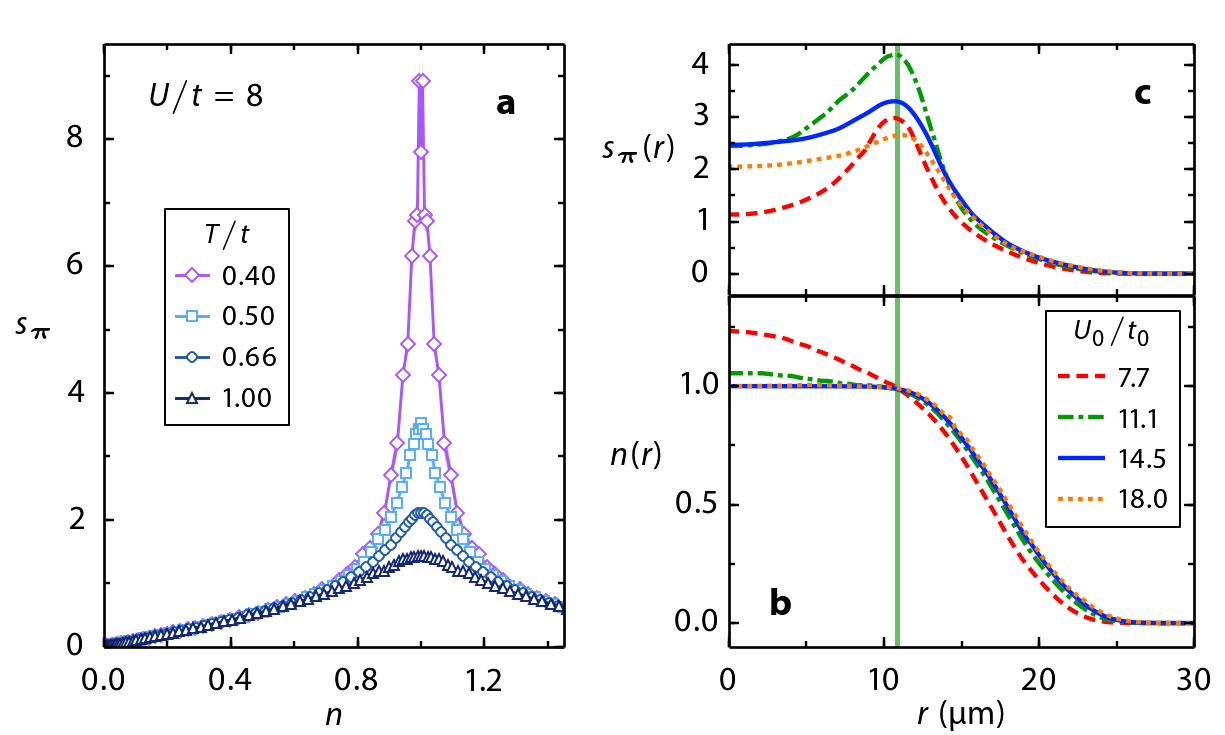
\includegraphics[width=0.8\columnwidth]{../figures/afmpaper/Hulet_fig3.png}
\caption{\textbf{Numerical calculations.} \textbf{a}, DQMC calculation of the
spin structure factor per lattice site as a function of density in a
homogeneous lattice for several temperatures.  $s_{\bv{\pi}}$ is sharply peaked
near $n=1$ and diverges as $T$ approaches $T_{N}$.  \textbf{b}, Density
profiles calculated at $T/t_{0}=0.6$ for different $U_{0}/t_{0}$. The atom
number used to obtain each profile maximizes the experimentally measured
$S_{\bv{\pi}}$, as will be explained in \S\ref{sec:number-vary}.  \textbf{c},
Profiles of the local spin structure factor $s_{\bv{\pi}}(r)$, for the same
conditions as in \textbf{b}.  The vertical green line in panels \textbf{b} and
\textbf{c} marks the radius at which $s_{\bv{\pi}}(r)$ is maximized for
$U_{0}/t_{0}=11.1$.}
\label{fig:bfig3}
\end{figure}

Figures.~\ref{fig:bfig3}b and~\ref{fig:bfig3}c show, respectively, the results
of numerical calculations of the local density and the local spin structure
factor in our trap, obtained as a function of distance from the center along a
body diagonal of the lattice.  For more details about these calculations refer
to Appendix~\ref{app:numerical}.  In Fig.~\ref{fig:bfig3}c we can see that the
local spin structure factor is maximized at the largest radius for which the
density is $n\approx1$.   

The finite extent of the lattice beams causes the lattice depth to decrease
with distance from the center, resulting in an increasing $t$, such that both
$U/t$ and $T/t$ decrease with increasing radius for constant $T$, as shown in
Fig.~\ref{fig:comp-inhomog}.  The radial decrease in $T/t$ causes
$s_{\bv{\pi}}(r)$  to maximize at the largest radius for which the density is
$n\approx1$.   For large $U_{0}/t_{0}$, where the cloud exhibits an $n=1$ Mott
plateau, this is the outermost radius of the plateau.  

\begin{figure}
\centering 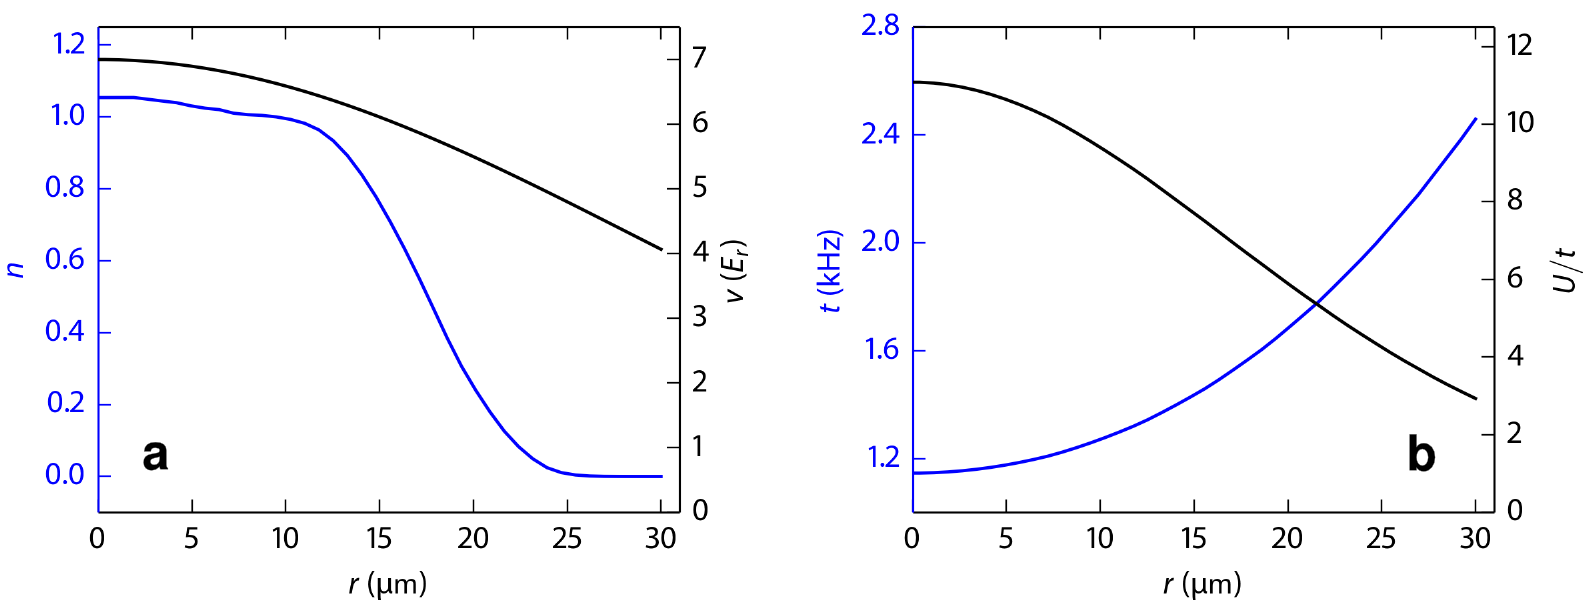
\includegraphics[width=125mm]{../figures/afmpaper/local-Hubbard.png}
\caption{\textbf{Local variation of the Hubbard parameters.}
\textbf{a}, The local value of the lattice depth $v$ (black line) is shown as a
function of distance from the center along a body diagonal of the lattice.  Due
to the finite extent of the lattice beams, $v$ varies across the density
profile (blue line),  which here is calculated for
$U_{0}/t_{0}=11.1$ at $T/t_{0}=0.60$.  \textbf{b},  The inhomogeneity in $v$
results in spatially varying Hubbard parameters $t$ (blue line) and $U/t$
(black line).} 
\label{fig:comp-inhomog}
\end{figure}

\section{Bragg signal optimization} 
\label{sec:number-vary}

One of the important technical aspects that we encountered with the Bragg
signal was the sensitivity to the number of atoms in the trap.  In the
experiment, we varied the atom number for each value of $U_{0}/t_{0}$ and found
that the Bragg signal had a maximum with respect to atom number.   The results
of this variation are shown in Fig.~\ref{fig:bfig03}.   According to the
picture presented in the previous section, varying the atom number optimizes
the size and location of the $n=1$ region of the cloud, in such a way that
\sPi\ is maximized.  

It is important to point out that the compensation also affects the density
distribution,  and there is an interplay between compensation and atom number.
Ideally one would want to vary both of them to find the absolute maximum of
\sPi.  In our experiment we found good results using a compensation
$g_{0}=3.7\,E_{r}$ for a lattice with depth $v_{0}=7\,E_{r}$.  This
compensation was the same for all values of $U_{0}/t_{0}$ that we studied.  

Besides adjusting the final value of the compensation to define the final
potential, we found it very important to dynamically adjust $g_{0}$ during the
lattice turn-on.  We believe that  this  adjustment reduces the time for the
system to equilibrate, by minimizing the deviation of the equilibrium density
distribution in the final potential from the starting density distribution in
the dimple trap prior to loading the lattice.   

\BraggFigureNum 

\section{Spin structure factor: results and thermometry}
 
\begin{figure}
\centering 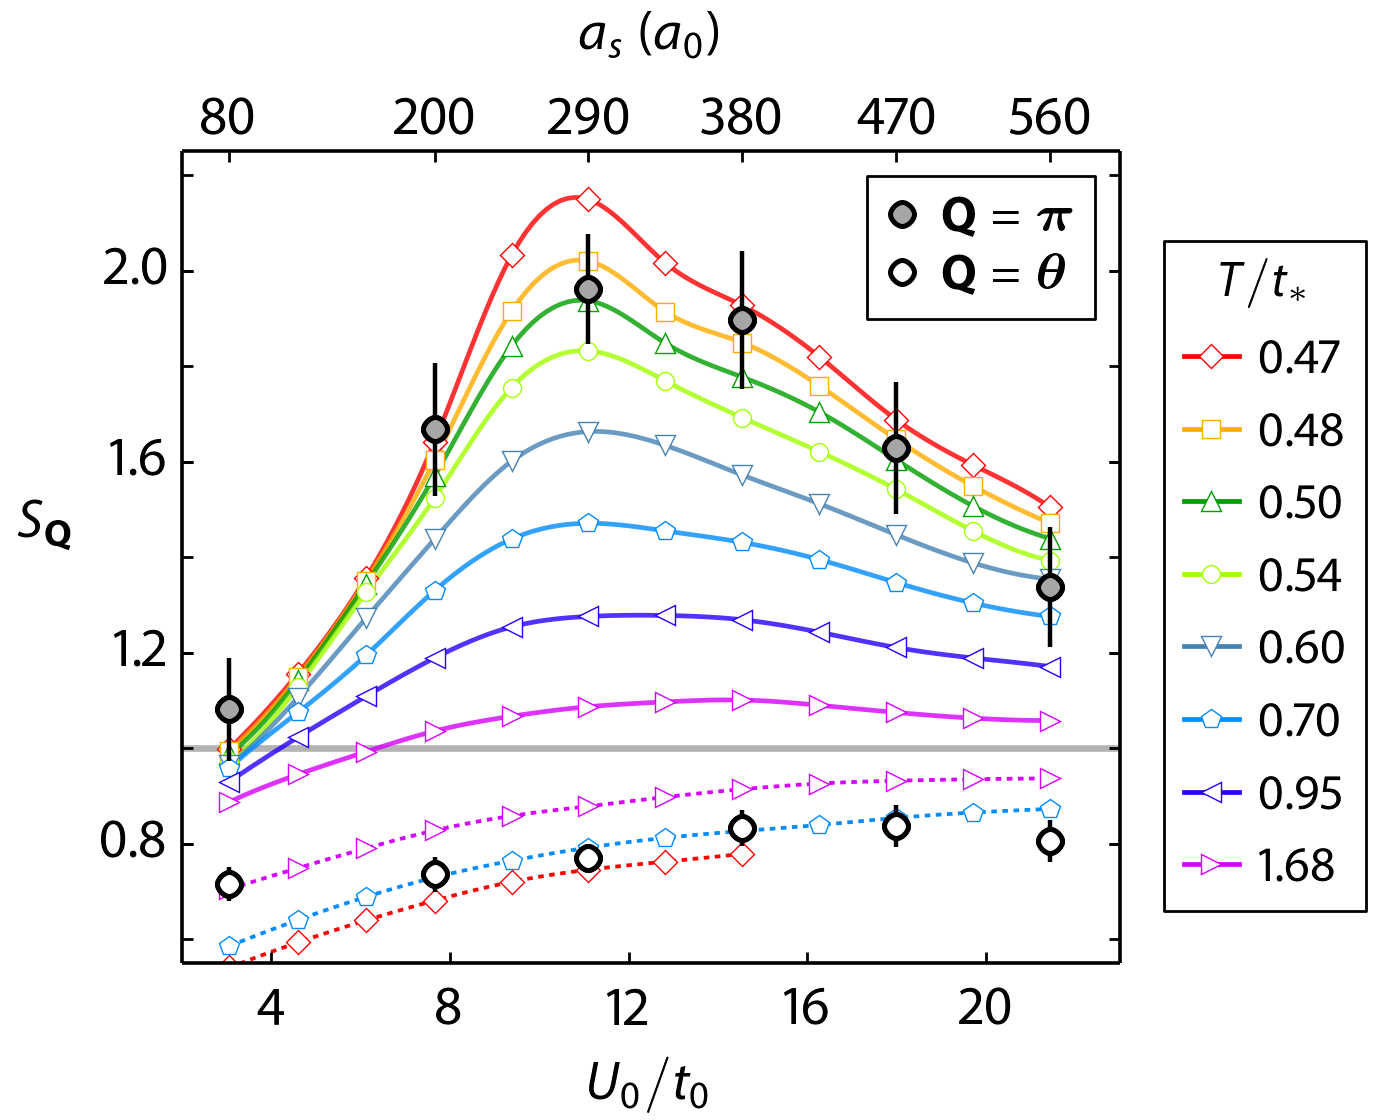
\includegraphics[width=105mm]{../figures/afmpaper/Hulet_fig4.png}
\caption{\textbf{Spin structure factor}  Measured $S_{\bv{\pi}}$ (filled
circles) and $S_{\bv{\theta}}$ (open circles) at optimized $N$ (see text) for
various $U_{0}/t_{0}$. The values of the $s$-wave scattering length
corresponding to $U_{0}/t_{0}$ for the experimental points are shown along the
top axis.  For each point at least 40 \textit{in-situ} and 40 time-of-flight
measurements of the scattered intensities are used to obtain the spin structure
factor.  Error bars are obtained from the SE of the scattered intensities; the
raw data for the scattered intensities is shown in Extended Data Fig.~5.
Numerical calculations of $S_{\bv{\pi}}$ (open symbols, lines as guide to the
eye) and $S_{\bv{\theta}}$ (open symbols, dashed lines as guide to the eye) for
various values of $T/t_{*}$. The numerical calculations for $S_{\bv{\theta}}$
are unreliable for $T/t_{*}>0.7$ and $U_{0}/t_{0}>15$.  $S_{\bv{\theta}}$
decreases slightly for weak interactions, where the fraction of double
occupancies increases.  }
\label{fig:bfig4} 
\end{figure}

Figure~\ref{fig:bfig4} shows the measured values of $S_{\bv{\pi}}$ and
$S_{\bv{\theta}}$ at optimal $N$ for various values of $U_{0}/t_{0}$.  We find
that $S_{\bv{\pi}}$ is peaked for $10 < U_{0}/t_{0} < 15$.  In contrast, the
measurements of $S_{\bv{\theta}}$ vary little over the full range of
interaction strengths, consistent with an absence of coherent Bragg scattering
in this direction.  Comparing the measured $S_{\bv{\pi}}$ with numerical
calculations for a homogeneous lattice (for example, those in
Fig.~\ref{fig:bfig3}a) allows us to set a trap independent upper limit on the
temperature, which we determine to be $T/t_{0}<0.7$.  

Precise thermometry is obtained by comparing the measured $S_{\bv{\pi}}$ with
numerical calculations averaged over the trap density distribution for
different values of $T$.  The results of such numerical calculations are also
shown in Fig.~\ref{fig:bfig4}, labeled by the value of $T/t_{*}$, which we
define as the local value of $T/t$ at the radius where the spin structure
factor per lattice site is maximal (see Fig.~\ref{fig:bfig3}a).  

At $U_{0}/t_{0}=11.1$, where measured AFM correlations are the largest, we find
$T/t_{*}=0.51\pm0.06$,  where the uncertainty is due to the statistical error
in the measured $S_{\bv{\pi}}$ and the systematic uncertainty in the lattice
parameters used for the numerical calculation.  This temperature is consistent
with the data at all values of $U_{0}/t_{0}$.  We caution, however, that for
values of $U/t>10$  a single-band Hubbard model may not be adequate, as
corrections involving higher bands may become
non-negligible~\cite{Werner2005,Mathy2009} (refer to
Fig.~\ref{fig:hubbardvalid}). 

 
As was shown in Fig.~\ref{fig:bfig3}c,  for $U_{0}/t_{0}=11.1$ the dominant
contribution to $S_{\bv{\pi}}$ comes from the outermost radius of the Mott
plateau. At that radius, the local value of $U/t$ is $U_{*}/t_{*}=9.1$,
consistent with DQMC calculations for the homogeneous
lattice~\cite{Staudt2000,Paiva2011,Kozik2013}, which find $T_{N}$ to be
maximized for $U/t$ between 8 and 9.  For $U_{0}/t_{0}=11.1$,
$t_{*}=1.3\,\mathrm{kHz}$, so we can infer the temperature of the system to be
$T=32\pm4\,\mathrm{nK}$.   In terms of $T_{N}$, the temperature is
$T/T_{N}=1.42\pm0.16$.   At this temperature, the numerical calculations
indicate that the correlation length is approximately equal to the lattice
spacing. 

\subsection{Optimal atom number} 

As was explained above, for each value of $U_{0}/t_{0}$ in
Fig.~\ref{fig:bfig4}, we varied the atom number to maximize \sPi.   The global
chemical potential $\mu_{0}$ must be increased, for larger $U_{0}/t_{0}$, to
guarantee the formation of a Mott plateau in the trap.   A larger $\mu_{0}$
results in a larger atom number,  hence the optimal value of $N$ increases with
$U_{0}/t_{0}$.  The value of $N$ corresponding to each $U_{0}/t_{0}$ point in
Fig.~\ref{fig:bfig4} is shown in Fig.~\ref{fig:number-EDfig2}. 

\begin{figure}
\centering 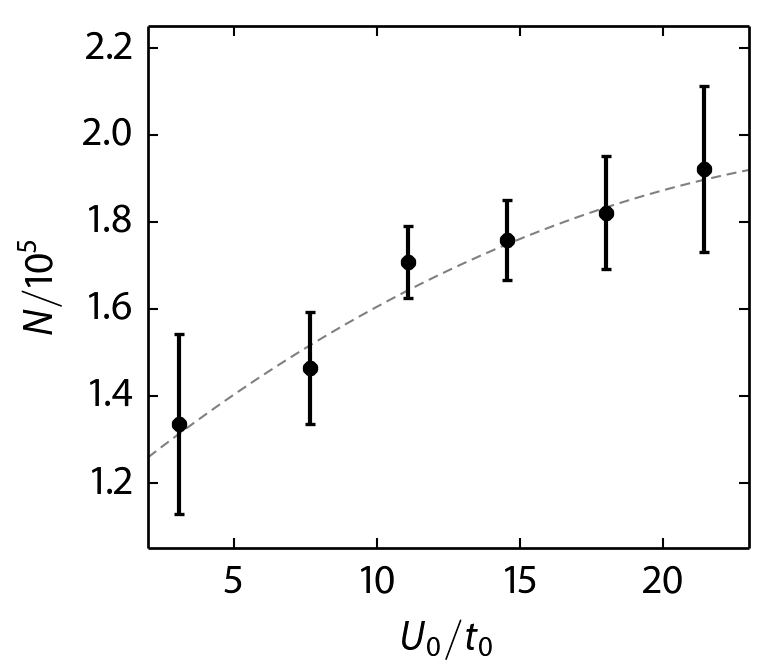
\includegraphics[width=75mm]{../figures/afmpaper/Hulet_EDfig2.png}
\caption{\textbf{Atom number for the data in Fig.~\ref{fig:bfig4}.}
Atom number $N$ which maximizes $S_{\bv{\pi}}$ as a function of $U_{0}/t_{0}$.
We control $N$ by adjusting the depth of the dimple trap.  Using a linear
calibration between the depth of the dimple trap and the final atom number  we
obtain the value of $N$ corresponding to the data in Fig.~4.  The error bars
correspond to the standard deviation of the dimple depths used in at least 40
\textit{in-situ} and 40 time-of-flight realizations of the experiment,
corresponding to the data in Fig.~4.   The line is a third order polynomial
fit, which is used to interpolate the value of $N$ for numerical calculations
shown in Fig.~4. }
\label{fig:number-EDfig2}
\end{figure}

\subsection{Decay of Bragg signal with hold time in the lattice}

\begin{figure}
\centering 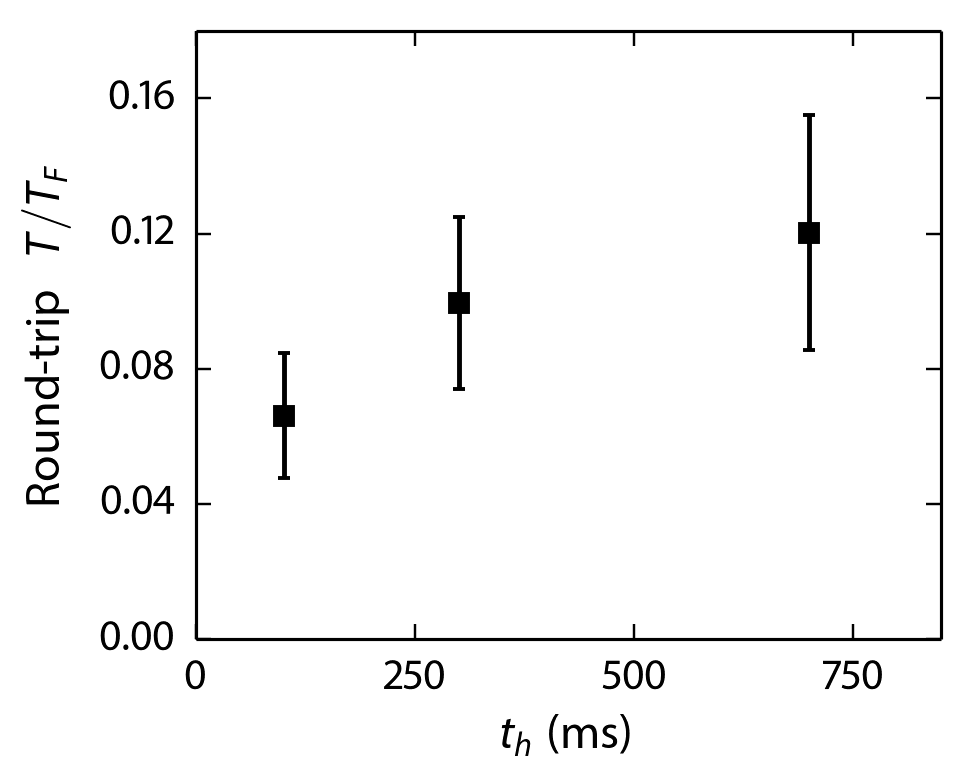
\includegraphics[width=75mm]{../figures/afmpaper/Hulet_EDfig3.png} 
\caption{\textbf{Round-trip temperature measurements.} Measurement of
the round-trip $T/T_{F}$ vs. hold time $t_{h}$ in a compensated lattice with
$v_{0}=7\,E_{r}$  and $g_{0}=3.7\,E_{r}$.  The duration of the loading ramps is
not included in $t_{h}$.  The scattering length is $326\,a_{0}$,  which
corresponds to $U_{0}/t_{0}=12.5$.  Error bars are the standard deviation of 6
independent realizations.  The temperature in the dimple trap before loading
into the lattice is $T/T_{F}=0.04\pm0.02$. }
\label{fig:roundtrip-heat}
\end{figure}


\begin{figure}
\centering 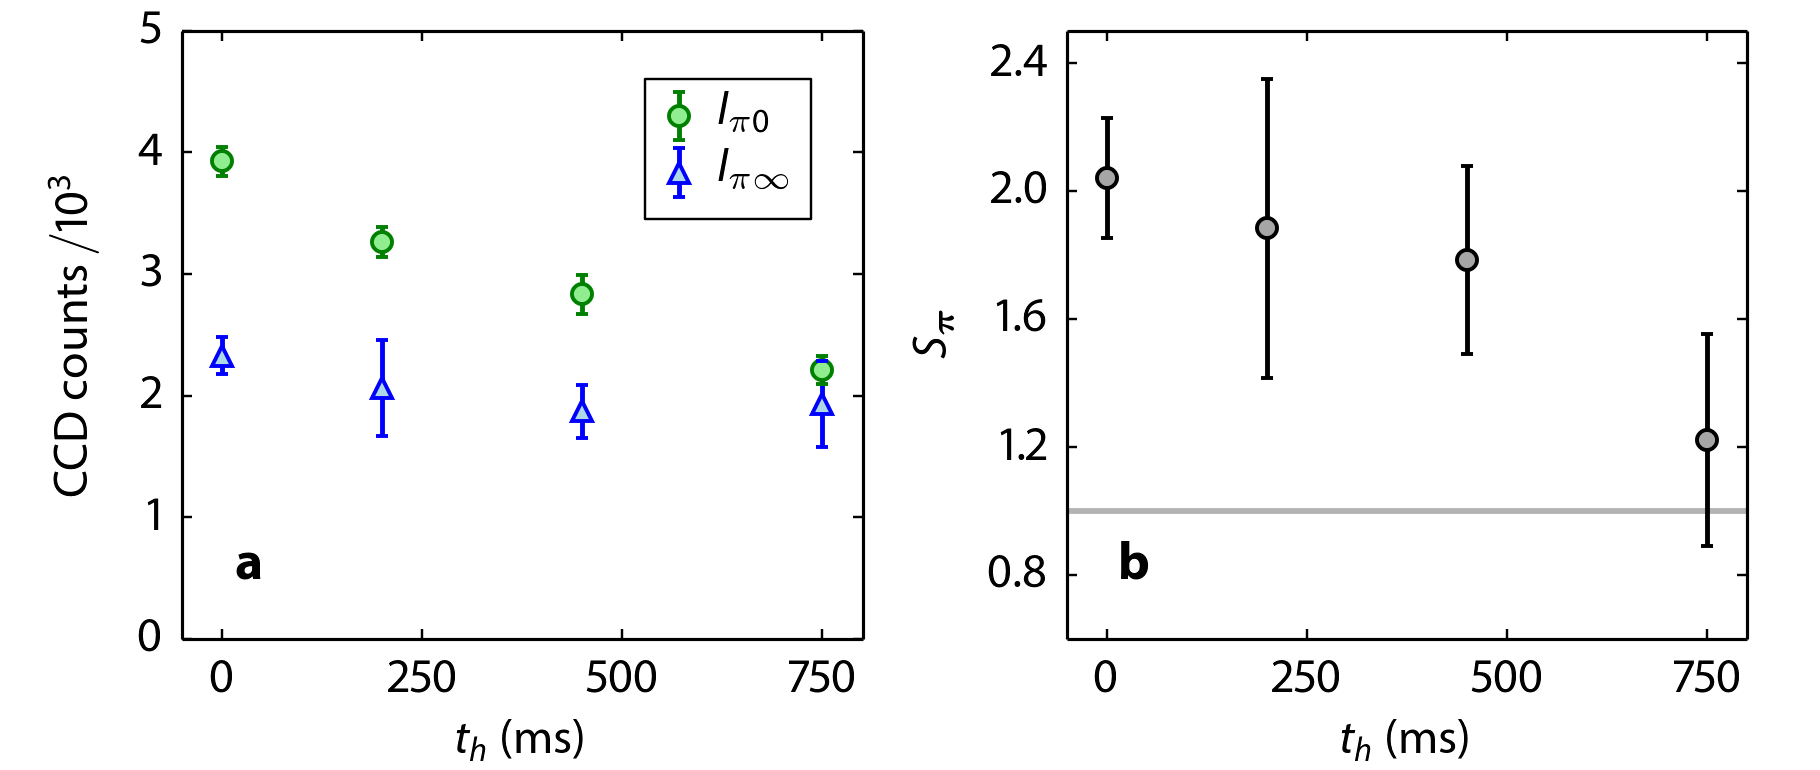
\includegraphics[width=135mm]{../figures/afmpaper/Hulet_EDfig4.png}
\caption{\textbf{Bragg signal decay with hold time.} \textbf{a}, Detected
counts vs. $t_{h}$, measured for momentum transfer $\mathbfsf{Q}=\bv{\pi}$ for
an \textit{in-situ} sample ($I_{\bv{\pi}0}$, green circles) and after decay of
the Debye-Waller factor ($I_{\bv{\pi}\infty}$, blue triangles).  For longer
hold times,  Bragg scattered intensity $I_{\bv{\pi}0}$ decays to match
$I_{\bv{\pi}\infty}$,  reflecting the absence of AFM correlations in a sample
at higher $T$.  \textbf{b}, The spin structure factor corresponding to the
scattered intensities shown in \textbf{a}.  For these measurements the
scattering length is $200\,a_{0}$, corresponding to $U_{0}/t_{0}=7.7$ in a
$7\,E_{r}$ deep lattice.  The compensation is $g_{0}=4.05\,E_{r}$, different
from that used for the data in Fig.~4.  The increased compensation requires a
larger atom number to realize an $n\simeq 1$ shell in the cloud.  The atom
number used here is $2.6\times10^{5}$ atoms.  The duration of the Bragg probe
is 2.7$\,\mu$s for these data.  Error bars in \textbf{a} are the standard error
of the mean of at least 5 measurements for $I_{\bv{\pi}\infty}$ and at least 10
measurements for $I_{\bv{\pi}0}$.  Error bars in \textbf{b} are obtained from
the uncertainty of the measured intensities.}
\label{fig:spidecay} 
\end{figure}

To probe the dependence of the spin structure factor on the temperature of the
sample, we do an experiment where we wait for a hold time $t_{h}$ in the
lattice before shining the Bragg probe.  To establish that the atoms heat up in
proportion to $t_{h}$, we measure the temperature in the dimple trap after a
lattice round-trip, as shown in Fig.~\ref{fig:roundtrip-heat}.  A lattice
round-trip consists of loading the atoms into the lattice and then reversing
the lattice loading ramps after a hold time $t_{h}$.  As expected for a system
with larger temperature, the measurements of the spin structure factor vs. hold
time, shown in Fig.~\ref{fig:spidecay}, indicate that AFM correlations decay as
expected for a hotter sample. 





\subsection{Entropy}


In Fig.~\ref{fig:bfig4} we compared the experimental measurements at various
$U_{0}/t_{0}$ with calculations at constant $T$.   Since ultracold atoms are
isolated systems, a constant value of the overall entropy per particle $S/(N
k_{\mathrm{B}})$ may be more appropriate for this comparison.  In any case,  we
find, from the results of the numerical calculations, that for
$10<U_{0}/t_{0}<15$, where AFM correlations are largest,  $S/(N
k_{\mathrm{B}})$ does not vary significantly with $U_{0}/t_{0}$, at constant
$T$.  This is shown in Fig.~\ref{fig:entropy-ED6}, where we plot the entropy
per particle $S/(Nk_{\mathrm{B}})$ corresponding to the constant $T$
calculations in Fig.~\ref{fig:bfig4}.  The fact that the entropy at constant
$T$ does not vary significantly with $U_{0}/t_{0}$, justifies the treatment
presented above at constant $T$. 
 
The calculations show that the entropy per particle in the trap for the range
of $U_{0}/t_{0}$ where \sPi\ is maximized,  is $S/(Nk_{\mathrm{B}})\simeq0.43$,
where $k_{\mathrm{B}}$ is the Boltzmann constant.  This entropy range is
consistent with $T/T_{F}=0.04\pm0.02$ measured in the harmonic dimple trap
before loading the atoms into the lattice~\cite{Kohl2006} and thus suggests
that the process of loading the atoms into the lattice is adiabatic. 

\begin{figure}
\centering 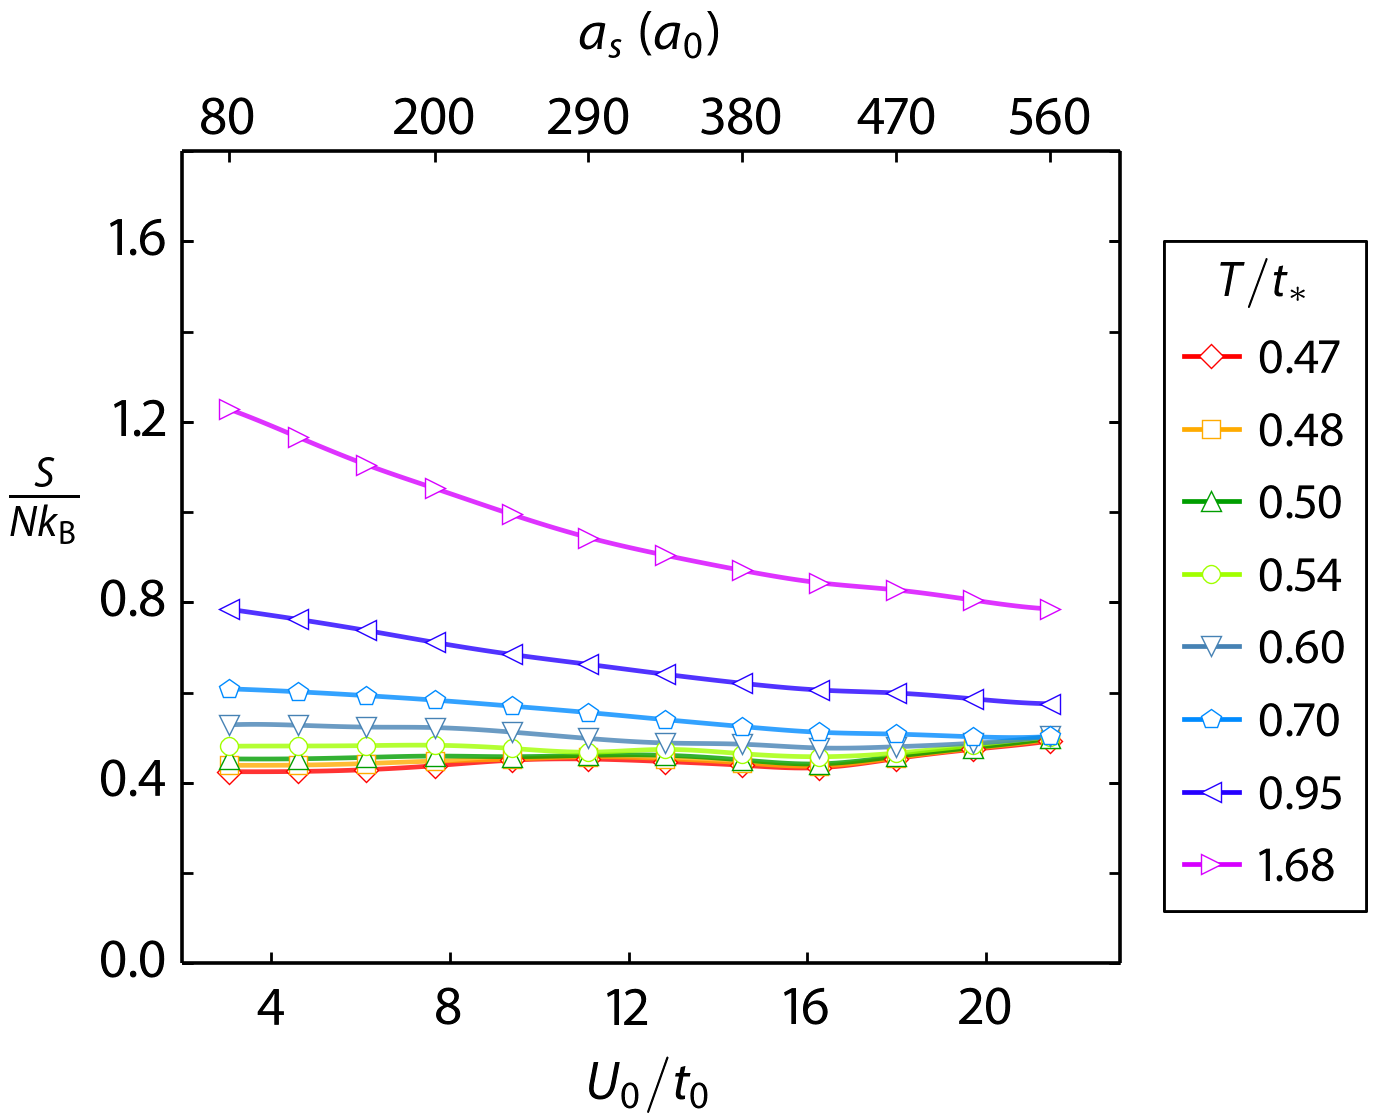
\includegraphics[width=80mm]{../figures/afmpaper/Hulet_EDfig6.png}
\caption{\textbf{Entropy per particle at constant $\bm{T}$.} Overall entropy
per particle $S/(Nk_{\mathrm{B}})$ as a function of $U_{0}/t_{0}$ for the
calculations at various $T/t_{*}$ shown in Fig.~\ref{fig:bfig4} (lines are
guides to the eye).  For the lowest temperatures, $S/(Nk_{\mathrm{B}})$ does
not vary significantly over the range of $U_{0}/t_{0}$ covered by the
experiment justifying the treatment at constant $T$.   A value of
$S/(Nk_{\mathrm{B}})\simeq0.43$ is obtained for the temperature determined from
the data in Fig.~4. This entropy is consistent with $T/T_{F}\simeq 0.04$,
measured in the harmonic dimple trap before loading the atoms into the
lattice.}
\label{fig:entropy-ED6}
\end{figure}


 

\section{Summary} 

We have observed AFM correlations in the Hubbard model using ultracold atoms in
an optical lattice via spin-sensitive Bragg scattering of light.  Because
magnetic order is extremely sensitive to $T$ in the vicinity of $T_{N}$,  Bragg
scattering provides precise thermometry in regimes previously inaccessible to
quantitative temperature measurements.  

In future studies our experimental setup can be configured to study the 2D
Hubbard model in an array of planes.  Further progress to lower temperature
will put is in a position to answer questions about competing pairing
mechanisms in 2D, and ultimately resolve the long standing question of $d$-wave
superconductivity in the Hubbard model.





%\subsection{Round-trip $T/T_{F}$ measurements.}  After loading the atoms
%into the $7E_{r}$ lattice we reverse the lattice loading ramps to return to
%the harmonic dimple trap and measure $T/T_{F}$.  When we compensate the
%lattice, such that the peak density is $n\simeq1$ throughout the ramps, the
%round-trip $T/T_{F}\simeq0.04$, the same value that we measure initially in the
%dimple trap.   In order to see any appreciable heating of the gas after
%round-trips we have to hold the atoms in the lattice for several hundred
%milliseconds.  For example, with $3.6E_{r}$ compensation after 700~ms the
%roundtrip temperature reaches $T/T_{F}=0.07(1)$.  With  $2E_{r}$
%compensation after 700~ms the round-trip temperature is $T/T_{F}=0.10(1)$. 




%\subsection{DQMC and NLCE calculations.}  DQMC and NLCE are used to calculate
%the local values of the thermodynamic quantities in our trap, including the
%density, entropy, and the spin structure factor.   
%
%DQMC results for a \parbox[b]{2.7em}{$6\!\!\times\!\!6\!\!\times\!\!6$} lattice
%were obtained with the methodology described in
%Refs.~\cite{PhysRevD.24.2278} and \cite{Paiva2010}.  Inverse temperature
%discretization $\Delta \tau = \beta/L=1/20t$ is sufficiently small that Trotter
%corrections are substantially less than statistical error bars.  Finite size
%effects were assessed by comparing DQMC results for
%\parbox[b]{2.7em}{$6\!\!\times\!\!6\!\!\times\!\!6$} and
%\parbox[b]{2.7em}{$8\!\!\times\!\!8\!\!\times\!\!8$} lattices.  Differences are
%only appreciable when the spin structure factor per lattice site,
%$s_{\bv{\pi}}>5$.  For the LDA results presented in Fig.~4 of the paper, the
%local value of $s_{\bv{\pi}}$ is always less than 4, so DQMC results with
%\parbox[b]{2.7em}{$6\!\!\times\!\!6\!\!\times\!\!6$} lattices are sufficient
%for the comparison with theory.  
%
%
%In NLCEs, an extensive property of the lattice model per site in the
%thermodynamic limit is expressed in terms of contributions from finite clusters
%that can be embedded in the lattice. NLCEs use the same basis as
%high-temperature expansions, however, properties of clusters are calculated via
%exact diagonalization, as opposed to a perturbative expansion in powers of the
%inverse temperature~\cite{Rigol2006,Tang2013}. The site-based NLCE for the
%Hubbard model~\cite{Khatami2011} is implemented here for a
%three-dimensional lattice and carried out to the eighth order.  Within its
%region of convergence ($T/t\gtrsim 1.5$ for any $n$ and $U$), NLCE results do
%not contain any systematic or statistical errors. The convergence region
%extends to significantly lower $T/t$ at $n=1$ and generally improves by
%increasing the interaction strength. At lower $T/t$, we take advantage of
%numerical resummations, such as Euler and Wynn transformations~\cite{Tang2013},
%to obtain an estimate. The NLCE provides a fast tool, which, given the value of
%$U/t$, generates results on a dense temperature and chemical potential grid in
%a single run. 
%
%DQMC calculations for any value of $n$ can be obtained reliably down to
%$T/t\approx0.36$ for $U/t < 8$.  For stronger interactions intermediate values
%of $n$ become inaccessible to DQMC due to the sign problem, in which case we
%rely on the NLCE to obtain values of the thermodynamic quantities for any value
%of $n$ down to temperatures as low as $T/t=0.40$.  

%\subsection{Local density approximation and comparison with theory.}  The local
%density approximation  was used to calculate the trap averaged $S_{\bv{\pi}}$
%and density profiles, starting from the DQMC and NLCE results and the known
%trapping potential.  It has been previously shown that the LDA agrees well with
%\textit{ab initio} DQCM simulations of the trapped Hubbard
%hamiltonian~\cite{Chiesa2011}.  Radial profiles for $U/t$ and the local chemical
%potential $\mu$ along a body diagonal of the lattice were used and spherical
%symmetry assumed.  
%
%When calculating density profiles we used the NLCE data sets. The density shows
%very little variation with temperature for $T/t<1$ so we only calculated
%density profiles at a single temperature value $T/t_{0} = 0.89$, see Fig.~3 in
%the text.  The NLCE density profiles were used to determine the global chemical
%potential such that for each value of $U_{0}/t_{0}$ in Fig.~4 we could
%calculate the trap averaged $S_{\bv{\pi}}$ using the atom number that was
%observed to peak up $S_{\bv{\pi}}$ as measured in the experiment (see Extended
%Data Fig. 3).
%


%\ExtFigTwo
%\ExtFigFour
